\lecture{14}{In-Context Learning over Graphs and Relational Transformers}{Tuesday, November 10, 2026}\label{ch:lec14}

% Local TikZ styles (prefix lec14)
\tikzset{
  lec14cap/.style={font=\scriptsize\sffamily, align=center},
  lec14lbl/.style={font=\scriptsize},
  lec14w/.style={circle, draw=black!80, fill=white, minimum size=1.5mm, inner sep=0pt},
  lec14h/.style={circle, draw=black!80, minimum size=1.8mm, inner sep=0pt},
  lec14t/.style={regular polygon, regular polygon sides=3, draw=black!80,
                 minimum size=2.7mm, inner sep=0pt},
  lec14dn/.style={rectangle, draw=black!80, minimum size=2.4mm, inner sep=0pt},
  lec14ln/.style={diamond, draw=black!80, minimum width=2.8mm, minimum height=3.8mm,
                  inner sep=0pt},
  lec14T/.style={{Stealth[length=1.4mm]}-{Stealth[length=1.4mm]}, ForestGreen!80!black,
                 semithick},
  lec14F/.style={{Stealth[length=1.4mm]}-{Stealth[length=1.4mm]}, BrickRed, semithick},
  lec14Q/.style={-{Stealth[length=1.4mm]}, Goldenrod!85!black, semithick, densely dashed},
  lec14gnn/.style={trapezium, trapezium angle=70, trapezium stretches=true,
                   draw=black!70,
                   fill=RoyalBlue!65, text=white, font=\tiny\sffamily\bfseries,
                   minimum width=9mm, minimum height=3.6mm, inner sep=1pt},
  lec14nn/.style={trapezium, trapezium angle=75, trapezium stretches=true,
                  draw=black!70, minimum width=9mm,
                  minimum height=9mm, inner sep=1pt},
  lec14blk/.style={block, font=\scriptsize\sffamily, minimum height=8mm},
  lec14att/.style={draw=black!60, rounded corners=3pt, fill=Goldenrod!35,
                   font=\scriptsize\sffamily, minimum width=30mm, minimum height=4.6mm,
                   inner sep=1pt},
  lec14mlp/.style={lec14att, fill=SkyBlue!35},
  lec14io/.style={draw=black!60, rounded corners=3pt, fill=Salmon!25, font=\scriptsize\sffamily,
                  align=center, minimum width=38mm, inner sep=2pt},
  lec14tab/.style={draw=black!80, thick, fill=white, font=\scriptsize\sffamily, align=left,
                   inner sep=2pt},
  lec14up/.style={black!50, -{Stealth[length=1.3mm]}},
  lec14fk/.style={thick, black!75, -{Stealth[length=1.5mm]}},
  lec14lnk/.style={thick, black},
  lec14dot/.style={circle, fill=black, minimum size=1.2mm, inner sep=0pt},
  lec14cell/.style={font=\scriptsize\sffamily, inner sep=0pt},
  lec14step/.style={circle, draw=black!70, fill=white, font=\tiny\sffamily\bfseries,
                    inner sep=0.5pt, minimum size=3mm},
}

\textbf{Outline.} Two talks. PRODIGY: ML paradigms and in-context learning $\to$
formulation of graph tasks as few-shot prompts $\to$ Prompt Graph (data graphs + task
graph) $\to$ in-context prediction GNN $\to$ in-context pretraining $\to$ results.
Relational Transformer (RT): RDL recap $\to$ relational foundation model $\to$ cell-level
tokenization, task-table integration, context sampling, relational attention $\to$
experiments and zero-shot results.

% ---------------------------------------------------------------------
\section{PRODIGY: in-context learning over graphs}\label{sec:lec14-prodigy}

\subsection{ML paradigms and in-context learning}\label{sec:lec14-icl}
\slides{4--11}

Huang, Ren, Chen, Krvzmanc, Zeng, Liang, Leskovec, \emph{PRODIGY: Enabling In-context
Learning Over Graphs}, NeurIPS 2023 (talk by Qian Huang).
\begin{itemize}
  \item \textbf{Different ML paradigms} (input \emph{hello}; outputs \emph{5}, \emph{h},
    \emph{bonjour}; \cref{fig:lec14-paradigms}):
    \begin{itemize}
      \item \textbf{Training:} a separate neural network per task;
      \item \textbf{Finetuning:} one shared (pretrained) network + a small head per task;
      \item \textbf{In-context learning:} one network for all tasks; the input is a
        \term{few-shot prompt} ``Thanks $\to$ merci, Wall $\to$ mur, hello $\to$'' and the
        output is \emph{bonjour}.
    \end{itemize}
\end{itemize}

\begin{figure}[htbp]
  \centering
  \begin{tikzpicture}[scale=0.85, transform shape]
    % training
    \foreach \x/\col/\out in {0/Salmon/5, 1.1/Peach/h, 2.2/LimeGreen/bonjour} {
      \node[lec14nn, fill=\col!55] (n) at (\x,0) {};
      \node[lec14lbl] (o) at (\x,1.05) {\emph{\out}};
      \node[lec14lbl] (i) at (\x,-1.0) {\emph{hello}};
      \draw[lec14up] (i) -- (n); \draw[lec14up] (n) -- (o);
    }
    \node[font=\scriptsize\sffamily\bfseries] at (1.1,-1.65) {Training};
    \draw[black!40] (3.0,-1.8) -- (3.0,1.4);
    % finetuning
    \begin{scope}[xshift=4.5cm]
      \node[lec14nn, fill=CornflowerBlue!45, minimum width=15mm, minimum height=8mm]
        (b) at (0,-0.2) {};
      \foreach \x/\col/\out in {-0.75/Salmon/5, 0/Peach/h, 0.75/LimeGreen/bonjour} {
        \node[lec14nn, fill=\col!55, minimum width=5mm, minimum height=3.5mm] (hd)
          at (\x,0.65) {};
        \node[lec14lbl] (o) at (\x,1.15) {\emph{\out}};
        \draw[lec14up] (b.north) -- (hd.south); \draw[lec14up] (hd) -- (o);
      }
      \node[lec14lbl] (i) at (0,-1.0) {\emph{hello}};
      \draw[lec14up] (i) -- (b);
      \node[font=\scriptsize\sffamily\bfseries] at (0,-1.65) {Finetuning};
    \end{scope}
    \draw[black!40] (6.0,-1.8) -- (6.0,1.4);
    % in-context learning
    \begin{scope}[xshift=8.0cm]
      \node[lec14nn, fill=RoyalBlue!65, minimum width=16mm, minimum height=12mm]
        (b) at (0,0.1) {};
      \node[lec14lbl] (o) at (0,1.15) {\emph{bonjour}};
      \node[lec14lbl, draw=red, thick, align=left, inner sep=2pt] (i) at (0,-1.0)
        {\emph{Thanks $\to$ merci} \quad \emph{hello $\to$}\\\emph{Wall $\to$ mur}};
      \draw[lec14up] (i) -- (b); \draw[lec14up] (b) -- (o);
      \node[font=\scriptsize\sffamily\bfseries] at (0,-1.65) {In-context learning};
      \node[lec14cap, text=red, anchor=west] at (1.85,-1.0) {few-shot\\prompting};
    \end{scope}
  \end{tikzpicture}
  \caption{Different machine learning paradigms (slides~6--8).}
  \label{fig:lec14-paradigms}
\end{figure}
\begin{definition}[In-context learning]\label{def:lec14-icl}
  \term{In-context learning}: performing a new task by ``learning'' from the input context
  \textbf{w/o gradient update}. Very powerful --- we only need \textbf{one foundation
  model} directly answering all tasks now!
\end{definition}
\begin{itemize}
  \item Examples (slide~9): \textbf{predicting sum} ($5+8=13$, $7+2=9$, $1+0=1$, $3+4=7$,
    $5+9=14$, $9+8=\,$\fbox{17}); \textbf{unscrambling} (gaot $\Rightarrow$ goat, sakne
    $\Rightarrow$ snake, brid $\Rightarrow$ bird, fsih $\Rightarrow$ fish, dcuk
    $\Rightarrow$ duck, cmihp $\Rightarrow$ \fbox{chimp}); \textbf{translating} (thanks
    $\Rightarrow$ merci, hello $\Rightarrow$ bonjour, mint $\Rightarrow$ menthe, wall
    $\Rightarrow$ mur, otter $\Rightarrow$ loutre, bread $\Rightarrow$ \fbox{pain}).
  \item Few-shot prompting over text vs.\ \textbf{what is in-context learning over
    graphs?} (slides~10, 14).
  \item \textbf{Today's plan:} formulate and enable \textbf{in-context learning over
    graphs}. \term{PRODIGY}: an in-context learner for graphs able to solve \textbf{novel
    tasks} on \textbf{novel graphs}:
    \begin{itemize}
      \item \textbf{Prompt Graph representation:} represent the few-shot prompt for
        different graph tasks in the \textbf{same input format}, so that it can be
        consumed by one shared model;
      \item \textbf{Prompt Graph inference:} in-context prediction GNN;
      \item \textbf{Pretraining:} generate diverse pretraining tasks in the format of
        PromptGraph (Neighbor Matching, MultiTask).
    \end{itemize}
\end{itemize}

\subsection{Formulation: few-shot prompts over graphs}\label{sec:lec14-formulation}
\slides{12--17}

\begin{itemize}
  \item \textbf{Graph learning tasks:} node classification, link prediction, graph
    classification (pictures: a social network; a knowledge graph with Wikidata,
    Freebase, ConceptNet, NELL, DBpedia, YAGO, \dots; molecules labelled
    toxic/non-toxic, approved/not approved).
  \item \textbf{Link prediction example} (few-shot prompting over graph for link
    classification):
    \begin{itemize}
      \item graph $\mathcal{G}$ (\emph{different graphs});
      \item \textbf{prompt examples} $\mathcal{S}$: input $x$ = (head, tail) node pair
        $\to$ label $y$ (one of two classes); \textbf{queries} $\mathcal{Q}$: (head, tail)
        $\to$ which label? (\emph{different tasks}, as in few-shot prompting over text).
    \end{itemize}
\end{itemize}
\begin{keyidea}
  An in-context learner for graphs should be able to solve \textbf{novel tasks on novel
  graphs without gradient updates}.
\end{keyidea}
\textbf{But, how to achieve this? Two challenges:}
\begin{enumerate}
  \item How to represent the few-shot prompt for \textbf{different graph tasks} in the
    \textbf{same input format}, so that it can be consumed by one shared model?\\
    $\Rightarrow$ \term{Prompt Graph}: represent each few-shot prompt over graph as a
    \textbf{meta hierarchical graph}.
  \item How to \textbf{pretrain} a model that can solve any task in this format?\\
    $\Rightarrow$ \term{PGPretraining}: pretrain a message passing model over
    self-supervised tasks in PromptGraph format with diverse underlying structures.
\end{enumerate}

\subsection{Prompt Graph and step 1: data graphs}\label{sec:lec14-pg}
\slides{18--24}

\begin{definition}[Prompt Graph]\label{def:lec14-pg}
  \term{Prompt Graph}: a unified representation of few-shot prompts over graph for diverse
  tasks (\cref{fig:lec14-pg}). Two levels:
  \begin{itemize}
    \item \textbf{data graphs} $\mathcal{G}^d$: one per prompt example in $\mathcal{S}$
      and per query in $\mathcal{Q}$ (step~1);
    \item \textbf{task graph}: one \term{data node} $v_x$ per data graph and one
      \term{label node} $v_y$ per label (step~2).
  \end{itemize}
  Legend: input nodes (head: circles, tail: triangles), data nodes (squares), label nodes
  (diamonds).
\end{definition}
\textbf{Step 1: Data Graph.}
\begin{itemize}
  \item \term{Data Graph} contextualizes each \textbf{input $x$} in the graph
    $\mathcal{G}$ (e.g.\ by \textbf{subgraph extraction}).
  \item \textbf{Link prediction:} subgraph around the (head, tail) pair;
    \textbf{node classification:} subgraph around the input node; \textbf{graph
    classification:} the input graph itself (its nodes are the input nodes).
  \item \textbf{DataGraph construction unifies the input format:}
    \begin{itemize}
      \item use a different \textbf{input node set} for classification over different
        levels (nodes vs edge vs graph);
      \item use \textbf{text feature} to unify features over different datasets.
    \end{itemize}
\end{itemize}

\subsection{Step 2: task graph}\label{sec:lec14-tg}
\slides{25--36}

\begin{itemize}
  \item \term{Task Graph} interconnects inputs and labels across examples to form
    context for queries (nodes $v_x$, $v_y$ as in \cref{def:lec14-pg}).
  \item \textbf{Edges} (link prediction, slides~26--32):
    \begin{itemize}
      \item \textbf{prompt examples:} \textbf{bidirectional edges between data nodes and
        all label nodes} (to the true label: T, to the other labels: F);
      \item \textbf{queries:} \textbf{single directed edges from each label to each data
        node} (marked ?).
    \end{itemize}
  \item Same task graph for \textbf{node classification} (slide~33) and \textbf{graph
    classification} (slide~34); only the data graphs differ.
  \item \textbf{Flexibility of Task Graph} -- it unifies the classification task format:
    \begin{itemize}
      \item different number of \textbf{classes} $\to$ different number of \textbf{label
        nodes};
      \item different number of \textbf{prompt examples (i.e.\ shots)} and queries $\to$
        different number of \textbf{data nodes} as well as how they connect with label
        nodes;
      \item e.g.\ 2-shots prompt for 2-class classification (4 examples, 1 query, 2 label
        nodes); 1-shot prompt for 3-class classification (3 examples, 2 queries, 3 label
        nodes).
    \end{itemize}
  \item \textbf{Prompt Graph for in-context learning} (slide~36): in-context learning over
    graph $\Rightarrow$ \textbf{inductive link prediction over hierarchical graph}
    (predict the query--label edges).
    \begin{itemize}
      \item task graph: \textbf{reflects what is the task} using examples (commonalities and
        differences);
      \item data graphs: \textbf{capture all relevant information about the input}.
    \end{itemize}
\end{itemize}

\begin{figure}[htbp]
  \centering
  \begin{tikzpicture}[scale=0.85, transform shape]
    % bands
    \draw[rounded corners=4pt, fill=Peach!15, draw=Peach!60!black] (-2.0,-1.6) rectangle (8.5,0.95);
    \draw[rounded corners=4pt, fill=CornflowerBlue!12, draw=CornflowerBlue!70!black] (-2.0,1.75) rectangle (8.5,4.05);
    \node[lec14cap, anchor=west, align=left] at (-1.9,0) {Data\\Graphs};
    \node[lec14cap, anchor=west, align=left] at (-1.9,2.9) {Task\\Graph};
    % data graphs, data graph encoders, data nodes
    \foreach \x/\col [count=\i] in {0/ForestGreen, 1.8/Brown, 3.6/Goldenrod, 5.4/Magenta,
                                    7.4/RoyalBlue} {
      \begin{scope}[shift={(\x,0)}]
        \draw[black!60, densely dotted, thick] (0,0) circle (0.72);
        \node[lec14w] (a) at (-0.38,0.22) {};
        \node[lec14w] (b) at (0.08,0.42) {};
        \node[lec14w] (c) at (0.4,0.05) {};
        \node[lec14w] (m) at (0.0,0.0) {};
        \node[lec14h, fill=\col] (e) at (-0.32,-0.34) {};
        \node[lec14t, fill=\col] (f) at (0.3,-0.38) {};
        \draw[black!70] (a)--(b) (b)--(c) (a)--(m) (m)--(c) (m)--(e) (m)--(f) (e)--(f) (c)--(f);
      \end{scope}
      \node[lec14gnn] (g\i) at (\x,1.33) {GNN};
      \node[lec14dn, fill=\col] (d\i) at (\x,2.15) {};
      \draw[black!50, densely dotted] (\x,0.72) -- (g\i.south);
      \draw[lec14up] (g\i.north) -- (d\i.south);
    }
    \node[lec14lbl] at (-0.8,0.62) {$\mathcal{G}^d$};
    % label nodes
    \node[lec14ln, fill=Peach] (yo) at (2.4,3.6) {};
    \node[lec14ln, fill=CornflowerBlue] (yb) at (4.8,3.6) {};
    \node[lec14lbl, left=1pt of yo] {$v_y$};
    \node[lec14lbl, left=1pt of d1] {$v_x$};
    % task-graph edges
    \draw[lec14T] (d1) -- (yo); \draw[lec14T] (d2) -- (yo);
    \draw[lec14T] (d3) -- (yb); \draw[lec14T] (d4) -- (yb);
    \draw[lec14F] (d1) -- (yb); \draw[lec14F] (d2) -- (yb);
    \draw[lec14F] (d3) -- (yo); \draw[lec14F] (d4) -- (yo);
    \draw[lec14Q] (yo) -- (d5); \draw[lec14Q] (yb) -- (d5);
    \node[font=\scriptsize\sffamily\bfseries, ForestGreen!80!black] at (0.85,3.0) {T};
    \node[font=\scriptsize\sffamily\bfseries, BrickRed] at (1.0,2.2) {F};
    \node[font=\scriptsize\sffamily\bfseries, Goldenrod!85!black] at (6.55,3.15) {?};
    % task-graph GNN and logits
    \node[lec14gnn, minimum width=40mm, minimum height=5.5mm,
          font=\scriptsize\sffamily\bfseries] (att) at (3.6,4.65) {GNN with attention};
    \node[lec14cap, anchor=west] at (6.0,4.65)
      {logit $=$ cosine\_similarity$(h_{\mathrm{label}}, h_{\mathrm{data}})$};
    % braces
    \draw[decorate, decoration={brace, mirror, amplitude=4pt}, thick]
      (-0.7,-0.88) -- (6.1,-0.88) node[midway, below=4pt, lec14cap] {Prompt examples $\mathcal{S}$};
    \node[lec14cap] at (7.4,-1.18) {Queries $\mathcal{Q}$};
  \end{tikzpicture}
  \caption{Prompt Graph for link prediction (slides~19--32) with the in-context prediction
  GNN on top (slides~40--42). T/F: prompt-example edges; ?: query edges.}
  \label{fig:lec14-pg}
\end{figure}

\subsection{Prompt Graph inference: in-context prediction GNN}\label{sec:lec14-gnn}
\slides{37--42}

\begin{itemize}
  \item Model: PromptGraph (task graph + data graphs) $\to$ Model $\to$ \textbf{scores}
    for the ? edges.
  \item \textbf{Hierarchical message passing over PromptGraph} (\cref{fig:lec14-pg}):
    \begin{enumerate}
      \item \textbf{Data Graph Encoder:} a GNN on each data graph $\mathcal{G}^d$ $\to$
        embedding of its data node;
      \item \textbf{Message passing over Task Graph:} \textbf{GNN with attention} over data
        and label nodes;
      \item \textbf{Compute logits}, e.g.\ for the query (head, tail) $\to$ ? (blue label):
    \end{enumerate}
\end{itemize}
\begin{equation}\label{eq:lec14-logit}
  \mathrm{logit} = \mathrm{cosine\_similarity}\big(h_{\mathrm{label}},\, h_{\mathrm{data}}\big)
\end{equation}

\subsection{PRODIGY pretraining}\label{sec:lec14-pretrain}
\slides{43--51}

\begin{itemize}
  \item \textbf{In-context pretraining:} we want to generate pretraining tasks in the
    format of \textbf{PromptGraph} and pretrain our model over them: Pretraining
    Data/Graph $\xrightarrow{\text{Data Gen}}$ PromptGraph $\to$ Model $\to$ Optimize Loss.
  \item \textbf{Pretraining data generation}, two stages (\cref{fig:lec14-pretrain}):
    \begin{enumerate}
      \item \textbf{few-shot prompt generation} (Neighbor Matching + MultiTask) $\to$
        graph $\mathcal{G}$, prompt examples $\mathcal{S}$, queries $\mathcal{Q}$;
      \item \textbf{convert to PromptGraph} (PromptGraph with augmentation).
    \end{enumerate}
  \item \term{MultiTask}: simply select multiple tasks for pretraining $\to$
    \textbf{supervised pretraining}.
  \item \term{Neighbor Matching}: \textbf{self-supervised pretraining}. Idea: the task is
    to \textbf{classify which neighborhood a node is in}, where each neighborhood is
    defined by other nodes in it.
    \begin{itemize}
      \item Slide~49: label nodes = two neighborhoods (\textbf{2 hops neighbors}, orange
        and blue); prompt examples: nodes with data graphs $\mathcal{G}_1^d,
        \mathcal{G}_2^d$ $\to$ orange, $\mathcal{G}_3^d, \mathcal{G}_4^d$ $\to$ blue;
        queries: a new node $\to$ orange? / blue?
    \end{itemize}
\end{itemize}
\begin{keyidea}
  \textbf{Mixing different data generation pipelines} gives more diverse pretraining data
  and better results!
\end{keyidea}
\textbf{In-context pretraining objectives} (slide~51):
\begin{itemize}
  \item \textbf{classification loss} over generated tasks;
  \item \textbf{attribute prediction loss}: reconstruct corrupted features during
    DataGraph augmentation.
\end{itemize}

\begin{figure}[htbp]
  \centering
  \begin{tikzpicture}[scale=0.85, transform shape]
    \node[lec14blk, fill=black!8] (src) at (0,0) {Pretraining\\Data/Graph};
    \node[lec14blk, fill=ForestGreen!25] (nm) at (2.7,0.6) {Neighbor\\Matching};
    \node[lec14blk, fill=ForestGreen!25] (mt) at (2.7,-0.6) {MultiTask};
    \node[lec14blk] (fs) at (5.5,0) {few-shot prompt\\$\mathcal{G}$, $\mathcal{S}$, $\mathcal{Q}$};
    \node[lec14blk, fill=CornflowerBlue!20] (pg) at (8.7,0) {PromptGraph\\(task graph +\\data graphs)};
    \node[lec14blk, fill=RoyalBlue!30] (m) at (11.0,0) {Model};
    \node[lec14blk] (l) at (13.1,0) {Optimize loss};
    \draw[arrow] (src.east) -- (nm.west);
    \draw[arrow] (src.east) -- (mt.west);
    \draw[arrow] (nm.east) -- (fs.west);
    \draw[arrow] (mt.east) -- (fs.west);
    \draw[arrow] (fs.east) -- (pg.west);
    \draw[arrow] (pg.east) -- (m.west);
    \draw[arrow] (m.east) -- (l.west);
    \node[lec14cap, BrickRed] at (2.7,1.3) {self-supervised};
    \node[lec14cap, BrickRed] at (2.7,-1.3) {supervised};
    \node[lec14cap, font=\scriptsize\sffamily\bfseries] at (4.1,1.9)
      {stage 1: few-shot prompt generation};
    \node[lec14cap, font=\scriptsize\sffamily\bfseries] at (8.2,1.25)
      {stage 2: convert to PromptGraph\\(with augmentation)};
    \node[lec14cap, align=left, anchor=north] at (13.1,-0.55)
      {classification loss\\+ attribute\\prediction loss};
  \end{tikzpicture}
  \caption{PRODIGY in-context pretraining: data generation in two stages, then the model is
  trained on the generated PromptGraphs (slides~44--51).}
  \label{fig:lec14-pretrain}
\end{figure}

\subsection{Experimental setup}\label{sec:lec14-setup}
\slides{52--54}

\begin{itemize}
  \item \textbf{Pretraining datasets (2):} \textbf{MAG240M}, a large scale citation
    network; \textbf{Wiki}, a knowledge graph constructed from Wikipedia (Xiong et al.,
    2018b).
  \item After pretraining, evaluate the \textbf{in-context learning performance} on
    diverse classification tasks over downstream graphs: \textbf{paper category
    prediction} (arXiv); \textbf{KG link prediction} (FB15K-237, NELL, ConceptNet).
  \item \textbf{Three baselines:}
    \begin{itemize}
      \item \textbf{NoPretrain}: randomly-initialized model with the same architecture as
        the pretrained models;
      \item \textbf{Contrastive}: standard contrastive learning with the same augmentation
        + a hard-coded nearest neighbor algorithm to adapt to the in-context learning
        setting;
      \item \textbf{Finetune}: trains an additional linear classification head on top of
        the graph encoder pretrained with contrastive learning.
    \end{itemize}
  \item \textbf{Three variants of PRODIGY} (different pretraining data generation):
    \textbf{PG-NM} (Neighbor Matching), \textbf{PG-MT} (Multi-task), \textbf{PG-ALL}
    (combines the two).
  \item \textbf{Graphs with different features:} use the \textbf{text embedding} provided
    by a pretrained language model (e.g.\ Bert).
\end{itemize}

\subsection{In-context learning results}\label{sec:lec14-results}
\slides{55--60}

\begin{table}[htbp]
  \centering\small
  \caption{Paper category classification: pretrain on MAG $\to$ in-context learning on
  arXiv (accuracy, best in bold as on slide~55; PG-NM / PG-MT shaded on the slide).}
  \label{tab:lec14-arxiv}
  \begin{tabular}{@{}cccccc|c@{}}
    \toprule
    Classes & NoPretrain & Contrastive & PG-NM & PG-MT & PRODIGY & Finetune\\
    \midrule
    3  & $33.16\pm0.30$ & $65.08\pm0.34$ & $72.50\pm0.35$ & $65.64\pm0.33$
       & $\mathbf{73.09\pm0.36}$ & $65.42\pm5.53$\\
    5  & $18.33\pm0.21$ & $51.63\pm0.29$ & $61.21\pm0.28$ & $51.97\pm0.27$
       & $\mathbf{61.52\pm0.28}$ & $53.49\pm4.61$\\
    10 & $9.19\pm0.11$  & $36.78\pm0.19$ & $46.12\pm0.19$ & $37.23\pm0.20$
       & $\mathbf{46.74\pm0.20}$ & $30.22\pm3.77$\\
    20 & $4.72\pm0.06$  & $25.18\pm0.11$ & $33.71\pm0.12$ & $25.91\pm0.12$
       & $\mathbf{34.41\pm0.12}$ & $17.68\pm1.15$\\
    40 & $2.62\pm0.02$  & $17.02\pm0.07$ & $23.69\pm0.06$ & $17.19\pm0.08$
       & $\mathbf{25.13\pm0.07}$ & $8.04\pm3.00$\\
    \bottomrule
  \end{tabular}
\end{table}

\begin{itemize}
  \item \textbf{Result 1:} PRODIGY improves performance in all cases, \textbf{up to 48\%}
    over contrastive and \textbf{3X} over Finetune (\cref{tab:lec14-arxiv}).
  \item \textbf{Result 2} (PG-NM column): PRODIGY can induce strong in-context learning
    with very different self-supervised pretraining tasks --- pretraining has no idea
    about classifying paper categories!
  \item \textbf{Result 3} (PRODIGY column): mixing different data generation pipelines
    gives more diverse pretraining data and better results!
  \item \textbf{Performance scaling with more shots} (ConceptNet, 4-way; accuracy vs.\
    shots 1--20): PG-ALL above Contrastive at every shot count ($\approx0.43\to0.63$ vs.\
    $\approx0.38\to0.51$, read off the plot). \textbf{Pretraining with only 3 shots
    $\Rightarrow$ the model can learn from context from much more than 3 shots!}
  \item \textbf{Data scaling} (accuracy vs.\ \# of training steps, $10^3$ to $\approx2\cdot
    10^4$, log scale): PG-ALL keeps rising ($\approx0.46\to0.61$), Contrastive fluctuates
    ($\approx0.43$--$0.53$). \textbf{Hard and diverse pretraining tasks generation pipeline
    allows the model to keep scaling with more training data.}
\end{itemize}

\subsection{Conclusion}\label{sec:lec14-prodigy-concl}
\slides{61}

PRODIGY enables \textbf{in-context learning over graphs} with a novel in-context task
representation, Prompt Graph, and corresponding pretraining architecture and objectives:
\begin{itemize}
  \item \textbf{Prompt Graph} provides a unified representation of few-shot prompts over
    graph for diverse tasks;
  \item \textbf{pretraining} a hierarchical message passing model over Prompt Graph enables
    in-context learning over unseen tasks on unseen graphs;
  \item \textbf{hard and diverse pretraining tasks} allow the model to keep scaling with
    more training data.
\end{itemize}

% ---------------------------------------------------------------------
\section{Relational Transformer}\label{sec:lec14-rt}

\subsection{Recap: relational deep learning}\label{sec:lec14-rdl}
\slides{62--66}

Talk ``Designing Transformers for Relational Data: Towards Foundation Models for
Forecasting over Relational Databases'' (Charilaos Kanatsoulis); paper: Ranjan, Hudovernik,
Znidar, Kanatsoulis et al., \emph{Relational Transformer: Toward Zero-Shot Foundation
Models for Relational Data}, 2025.
\begin{itemize}
  \item Slides~63--65 as in \cref{ch:lec12}: RDL [Fey et al.\ 2023] pipeline Relational DB
    $\to$ Graph Problem $\to$ Graph ML $\to$ Solutions; relational databases as
    entity-level graphs (\textbf{every entity (row) is a node}, \textbf{edges defined by
    foreign key--primary key links}); predictive tasks are graph ML problems: node-level
    (churn, life-time value), link-level (product affinity, recommendation), graph-level
    (fraud detection).
  \item \textbf{RDL architectures} (slide~66): RDL-GNN [Robinson et al.\ 2024], RelGNN
    [Cheng, C.K., Leskovec 2025], Relational Graph Transformer (RelGT) [Dwivedi, Jaladi,
    Shen, Lopez, C.K., et al.\ 2025] (both in \cref{ch:lec13}), RelLLM [Wu et al.\ 2025].
\end{itemize}

\subsection{Toward a relational foundation model}\label{sec:lec14-rfm}
\slides{67--69}

\begin{itemize}
  \item Slides~67--68 as in \cref{ch:lec13}: \textbf{disadvantages of end-to-end RDL}:
    (1) \textbf{schema- and task-specific}; (2) \textbf{limited transfer}: cannot
    generalize to new databases or tasks. \textbf{Goal:} bring the success of foundation
    models (LLMs, ViT) to relational data.
  \item \textbf{The promise of the relational foundation model} (slide~69):
    \begin{itemize}
      \item \textbf{zero-shot forecasting} $\to$ new databases, unseen tasks;
      \item \textbf{few-shot / fine-tuning} with limited supervision.
    \end{itemize}
  \item \textbf{Broader impact: democratize AI for structured data} (non-experts gain
    accessible predictive tools, experts gain strong pretrained initialization).
\end{itemize}

\subsection{Relational Transformer (RT): overview}\label{sec:lec14-rt-ov}
\slides{70}

\begin{keyidea}
  Treat \textbf{each database cell as a token} and model its relationships through
  \textbf{Relational Attention}.
\end{keyidea}
\begin{itemize}
  \item \textbf{Core innovations:} (1) \textbf{cell-level tokenization}, (2)
    \textbf{task-table integration}, (3) \textbf{Relational Attention}
    (\cref{fig:lec14-rt}).
  \item \textbf{(a) Schema:} database schema (User, Sale, Item) + \textbf{task schema} Task
    (Time, ItemID (F), Label) for the task definition ``Predict total sales over next
    week.''
  \item \textbf{(b) Context window:} cells of the User, Sale, Item, Task tables, each with
    its table name and column name; links follow the keys; \textbf{task rows provide
    in-context labels}; \textbf{target row with masked cell} (?).
  \item \textbf{(c) Architecture:} \textbf{set} of cell values $\to$ per-datatype encoder
    + frozen LM embedding $\to$ \textbf{Relational Transformer block} $\times N$
    (relational attention layers $\to$ full attention $\to$ MLP) $\to$ per-datatype decoder
    $\to$ \textbf{predicted cell value}.
\end{itemize}

\begin{figure}[htbp]
  \centering
  \begin{tikzpicture}[scale=0.85, transform shape]
    % (a) schema
    \node[lec14tab] (u) at (0,0) {\textbf{User}\\UserID (P)\\Gender};
    \node[lec14tab] (s) at (2.2,0) {\textbf{Sale}\\Time\\UserID (F)\\ItemID (F)\\Stars};
    \node[lec14tab] (i) at (4.4,0) {\textbf{Item}\\ItemID (P)\\Price\\Details};
    \node[lec14tab, draw=Plum!80!black, text=Plum!70!black] (t) at (6.7,0)
      {\textbf{Task}\\Time\\ItemID (F)\\Label};
    \begin{scope}[on background layer]
      \node[fill=black!10, fit=(u)(s)(i), inner sep=5pt,
            label={[lec14cap]above:Database schema}] (db) {};
    \end{scope}
    \draw[lec14fk] (s.west) -- (u.east);
    \draw[lec14fk] (s.east) -- (i.west);
    \draw[lec14fk, Plum] (t.west) -- (i.east);
    \node[lec14cap, text=Plum] at (6.7,-1.15) {Task schema};
    \node[lec14cap, draw=Plum, rounded corners=4pt, inner sep=3pt] at (4.6,1.95)
      {Task definition: ``Predict total sales over next week.''};
    \node[lec14cap] at (3.3,-1.75) {(P) = primary key \qquad (F) = foreign key};
    \node[font=\small\sffamily\bfseries] at (3.3,-2.4) {(a) Schema};
    % (c) architecture
    \begin{scope}[xshift=12.0cm]
      \node[lec14cap] (in) at (0,-3.45) {\textbf{Set} of cell values (target cell masked)};
      \node[lec14io] (enc) at (0,-2.45)
        {$\forall$ cells: per-datatype encoder \texttt{num|text|bool|time}\\
         + frozen LM embedding for ``\texttt{<column> of <table>}''};
      \node[lec14att] (col) at (0,-1.3) {Column Attention};
      \node[lec14att] (fea) at (0,-0.7) {Feature Attention};
      \node[lec14att] (nei) at (0,-0.1) {Neighbor Attention};
      \node[lec14mlp] (ful) at (0,0.5) {Full Attention};
      \node[lec14mlp] (mlp) at (0,1.1) {MLP};
      \node[draw=BurntOrange, very thick, rounded corners=4pt, fit=(col)(mlp),
            inner sep=4pt] (blk) {};
      \draw[lec14up] (in) -- (enc);
      \draw[lec14up] (enc) -- (blk.south);
      \draw[lec14up] (col) -- (fea);
      \draw[lec14up] (fea) -- (nei);
      \draw[lec14up] (nei) -- (ful);
      \draw[lec14up] (ful) -- (mlp);
      \node[lec14io] (dec) at (0,2.25) {per-datatype decoder \texttt{num|text|bool|time}};
      \draw[lec14up] (blk.north) -- (dec);
      \node[lec14cap] (out) at (0,2.95) {predicted cell value};
      \draw[lec14up] (dec) -- (out);
      \node[lec14cap, anchor=east, align=right] at (-2.35,0.75)
        {\textbf{Relational}\\\textbf{Transformer}\\\textbf{Block}\\(repeated\\$N$ times)};
      \draw[decorate, decoration={brace, amplitude=3pt}, thick]
        (-2.05,-1.5) -- (-2.05,0.1);
      \node[lec14cap, anchor=east, align=right] at (-2.25,-0.7)
        {Relational\\Attention\\Layers};
      \node[font=\small\sffamily\bfseries] at (0,-4.0) {(c) Architecture};
    \end{scope}
  \end{tikzpicture}
  \caption{Relational Transformer: (a) database schema + task schema; (c) architecture
  (slide~70).}
  \label{fig:lec14-rt}
\end{figure}

\subsection{Input representation and task label integration}\label{sec:lec14-input}
\slides{71--74}

Running example: tables Transactions, Products, Users linked by key columns.
\begin{itemize}
  \item \textbf{Prior work}, e.g.\ RDL-GNN, RelGNN, RelGT, RelLLM, \textbf{tokenize at the
    row-level} $\Rightarrow$ leads to \textbf{schema-specific architectures}.
  \item \term{Cell-level tokenization}: one token per cell:
\end{itemize}
\begin{equation}\label{eq:lec14-token}
  \text{token} = (\text{value},\ \text{column},\ \text{table})
\end{equation}
\begin{itemize}
  \item Table is a MiniLMv2 description of the table; column is a MiniLMv2 text
    description of the column.
  \item \textbf{Benefits:} \textbf{unifies relational databases of any schema into a
    consistent input space}; \textbf{leverages cell-to-cell dependencies}.
  \item \textbf{Task label integration} (slide~74): the task is a table too (e.g.\
    \textbf{User-Churn} with columns Fkey, Val., Time; Fkey $\to$ Users), tokenized at the
    cell level. \textbf{Benefits:} cast \textbf{any node-level task as masked token
    prediction (MTP)}; adds \textbf{autoregressive labels} for task tokens.
\end{itemize}
\begin{caution}
  Slide~73 says ``Column is a MiniLMv2 text description of the \emph{table}''; correct: of the
  \emph{column} (slide~70: LM embedding for ``\texttt{<column> of <table>}'').
\end{caution}

\subsection{Context sampling}\label{sec:lec14-sampling}
\slides{75--81}

\textbf{Sampling rules} (wording of slides~76--81, \cref{fig:lec14-sampling}):
\begin{enumerate}
  \item sample \textbf{seed node} and \textbf{hide value};
  \item always \textbf{include parent} nodes (F $\to$ P keys);
  \item \textbf{subsample child rows} (P $\to$ F keys);
  \item only sample from \textbf{previous timestamps} $\Rightarrow$ \textbf{avoid temporal
    leakage}.
\end{enumerate}
Slide~75 words rules~2--3 as ``always \textbf{sample parent} nodes (F $\to$ P keys)'' and
``run \textbf{Breadth-First-Search} on children (P $\to$ F keys)''.
Walk-through (slides~76--81): seed = User-Churn row (Fkey 1, hidden value, time $t_0$)
$\to$ parent Users row (Pkey 1) $\to$ child Transactions rows (Fkey 1, Fkey 98) and (1,
100) $\to$ their parent Products rows (Pkey 98, 100) $\to$ earlier User-Churn row of user 1
with $t_1<t_0$.

\begin{figure}[htbp]
  \centering
  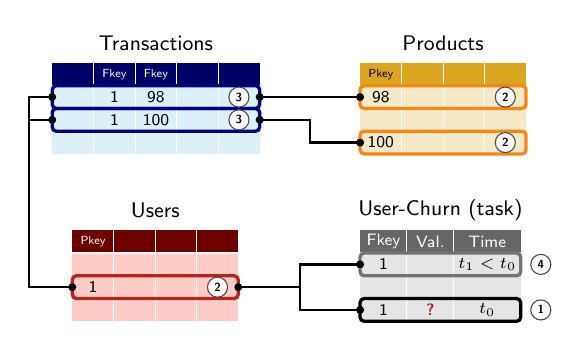
\begin{tikzpicture}[scale=0.85, transform shape]
    % ---------- Transactions ----------
    \begin{scope}[shift={(0,2.5)}]
      \fill[NavyBlue!80!black] (0,0) rectangle (3.1,-0.34);
      \fill[SkyBlue!30] (0,-0.34) rectangle (3.1,-1.36);
      \foreach \x in {0.62,1.24,1.86,2.48} \draw[white] (\x,0) -- (\x,-1.36);
      \foreach \y in {-0.34,-0.68,-1.02} \draw[white] (0,\y) -- (3.1,\y);
      \node[lec14cell, text=white, font=\tiny\sffamily] at (0.93,-0.17) {Fkey};
      \node[lec14cell, text=white, font=\tiny\sffamily] at (1.55,-0.17) {Fkey};
      \draw[very thick, NavyBlue, rounded corners=1.5pt] (0,-0.34) rectangle (3.1,-0.68);
      \draw[very thick, NavyBlue, rounded corners=1.5pt] (0,-0.68) rectangle (3.1,-1.02);
      \node[lec14cell] at (0.93,-0.51) {1}; \node[lec14cell] at (1.55,-0.51) {98};
      \node[lec14cell] at (0.93,-0.85) {1}; \node[lec14cell] at (1.55,-0.85) {100};
      \node[lec14step] at (2.79,-0.51) {3}; \node[lec14step] at (2.79,-0.85) {3};
      \node[font=\small\sffamily] at (1.55,0.3) {Transactions};
    \end{scope}
    % ---------- Products ----------
    \begin{scope}[shift={(4.6,2.5)}]
      \fill[Goldenrod] (0,0) rectangle (2.48,-0.34);
      \fill[Goldenrod!25] (0,-0.34) rectangle (2.48,-1.36);
      \foreach \x in {0.62,1.24,1.86} \draw[white] (\x,0) -- (\x,-1.36);
      \foreach \y in {-0.34,-0.68,-1.02} \draw[white] (0,\y) -- (2.48,\y);
      \node[lec14cell, font=\tiny\sffamily] at (0.31,-0.17) {Pkey};
      \draw[very thick, BurntOrange, rounded corners=1.5pt] (0,-0.34) rectangle (2.48,-0.68);
      \draw[very thick, BurntOrange, rounded corners=1.5pt] (0,-1.02) rectangle (2.48,-1.36);
      \node[lec14cell] at (0.31,-0.51) {98};
      \node[lec14cell] at (0.31,-1.19) {100};
      \node[lec14step] at (2.17,-0.51) {2}; \node[lec14step] at (2.17,-1.19) {2};
      \node[font=\small\sffamily] at (1.24,0.3) {Products};
    \end{scope}
    % ---------- Users ----------
    \begin{scope}[shift={(0.3,0)}]
      \fill[Maroon!85!black] (0,0) rectangle (2.48,-0.34);
      \fill[Salmon!40] (0,-0.34) rectangle (2.48,-1.36);
      \foreach \x in {0.62,1.24,1.86} \draw[white] (\x,0) -- (\x,-1.36);
      \foreach \y in {-0.34,-0.68,-1.02} \draw[white] (0,\y) -- (2.48,\y);
      \node[lec14cell, text=white, font=\tiny\sffamily] at (0.31,-0.17) {Pkey};
      \draw[very thick, BrickRed, rounded corners=1.5pt] (0,-0.68) rectangle (2.48,-1.02);
      \node[lec14cell] at (0.31,-0.85) {1};
      \node[lec14step] at (2.17,-0.85) {2};
      \node[font=\small\sffamily] at (1.24,0.3) {Users};
    \end{scope}
    % ---------- User-Churn (task table) ----------
    \begin{scope}[shift={(4.6,0)}]
      \fill[Gray!80!black] (0,0) rectangle (2.4,-0.34);
      \fill[Gray!20] (0,-0.34) rectangle (2.4,-1.36);
      \foreach \x in {0.7,1.4} \draw[white] (\x,0) -- (\x,-1.36);
      \foreach \y in {-0.34,-0.68,-1.02} \draw[white] (0,\y) -- (2.4,\y);
      \node[lec14cell, text=white] at (0.35,-0.17) {Fkey};
      \node[lec14cell, text=white] at (1.05,-0.17) {Val.};
      \node[lec14cell, text=white] at (1.9,-0.17) {Time};
      \draw[very thick, black!55, rounded corners=1.5pt] (0,-0.34) rectangle (2.4,-0.68);
      \draw[very thick, black, rounded corners=1.5pt] (0,-1.02) rectangle (2.4,-1.36);
      \node[lec14cell] at (0.35,-0.51) {1};
      \node[lec14cell] at (1.9,-0.51) {$t_1<t_0$};
      \node[lec14cell] at (0.35,-1.19) {1};
      \node[lec14cell, text=BrickRed] at (1.05,-1.19) {\textbf{?}};
      \node[lec14cell] at (1.9,-1.19) {$t_0$};
      \node[lec14step] at (2.7,-0.51) {4}; \node[lec14step] at (2.7,-1.19) {1};
      \node[font=\small\sffamily] at (1.2,0.3) {User-Churn (task)};
    \end{scope}
    % ---------- key links ----------
    \draw[lec14lnk] (3.1,1.99) -- (4.6,1.99);
    \draw[lec14lnk] (3.1,1.65) -- (3.85,1.65) |- (4.6,1.31);
    \draw[lec14lnk] (0,1.99) -- (-0.35,1.99) -- (-0.35,-0.85) -- (0.3,-0.85);
    \draw[lec14lnk] (0,1.65) -- (-0.35,1.65);
    \draw[lec14lnk] (2.78,-0.85) -- (3.7,-0.85) |- (4.6,-0.51);
    \draw[lec14lnk] (3.7,-0.85) |- (4.6,-1.19);
    \foreach \p in {(3.1,1.99), (4.6,1.99), (3.1,1.65), (4.6,1.31), (0,1.99), (0,1.65),
                    (0.3,-0.85), (2.78,-0.85), (4.6,-0.51), (4.6,-1.19)}
      \node[lec14dot] at \p {};
  \end{tikzpicture}
  \caption{Context sampled for a User-Churn seed row (slides~76--81); circled numbers =
  sampling rule that adds the row.}
  \label{fig:lec14-sampling}
\end{figure}

\subsection{Relational attention}\label{sec:lec14-attn}
\slides{82--85}

Three \term{relational attention} layers (followed by full attention and an MLP in each RT
block, \cref{fig:lec14-rt}). Slide~82 outlines the sampled context; slides~83--85 mark one
cell and outline the cells it attends to:
\begin{enumerate}
  \item \term{Column attention}: cells of the \textbf{same column} (slide~83: the masked
    User-Churn Val.\ cell $\leftrightarrow$ the Val.\ cells of the other User-Churn rows);
  \item \term{Feature attention}: cells of the \textbf{same row and its parent row}
    (slide~84: masked cell $\leftrightarrow$ its User-Churn row + the Users row it points
    to);
  \item \term{Neighbor attention}: cells of the \textbf{neighboring (child) rows} (slide~85:
    a Users cell $\leftrightarrow$ its own row + the 2 Transactions rows and the 2
    User-Churn rows that point to user 1).
\end{enumerate}

\subsection{Experimental setup and pretraining}\label{sec:lec14-rt-setup}
\slides{86--89}

\begin{itemize}
  \item \textbf{RelBench: 7 diverse datasets} (as in \cref{ch:lec12}): E-Commerce
    (rel-amazon, rel-avito, rel-hm), Social (rel-event, rel-stack), Sports (rel-f1),
    Medical (rel-trial).
  \item \textbf{Tasks:} binary classification and regression. \textbf{Pretraining:}
    \textbf{leave-one-database-out} pretraining. \textbf{Test} on unseen schema.
  \item \textbf{Baselines:}
    \begin{enumerate}
      \item \textbf{Griffin} [Wang et al.\ 2025]: a universal feature encoder followed by a
        GNN;
      \item \textbf{Gemma LLMs} [Wydmuch]: prompt Gemma3 with text-serialized database
        subgraph;
      \item \textbf{RDL-GNN} [Robinson et al.\ 2024]: schema specific GNN baseline.
    \end{enumerate}
  \item \textbf{RT pretraining} (slide~89): backbone \textbf{12 layers, 22M parameters};
    pre-training task: \textbf{Masked Token Prediction on RelBench}; training duration:
    \textbf{50k steps 8xA100}; \textbf{linear decoder}; objective: \textbf{Huber for
    regression, BCE for classification}.
\end{itemize}

\subsection{Results}\label{sec:lec14-rt-results}
\slides{90--94}

\begin{table}[htb]
  \centering\footnotesize
  \setlength{\tabcolsep}{3.5pt}
  \caption{Zero-shot transfer: test AUROC (\%) on RelBench classification tasks, by whether
  the target dataset is in pretraining; best per row in bold as on slide~92.}
  \label{tab:lec14-zs}
  \begin{tabular}{@{}llcccccccc@{}}
    \toprule
    \multicolumn{2}{@{}l}{Target dataset $\in$ pretraining? $\to$}
      & \multicolumn{3}{c}{Maybe} & \multicolumn{3}{c}{No} & \multicolumn{2}{c@{}}{Yes}\\
    \cmidrule(lr){3-5}\cmidrule(lr){6-8}\cmidrule(l){9-10}
    Dataset $\downarrow$ & Task $\downarrow$ & Gemma & Gemma & Gemma
      & \shortstack{Entity\\Mean} & Griffin & \shortstack{RT\\(ours)} & Griffin
      & \shortstack{RT\\(ours)}\\
    \multicolumn{2}{@{}r}{Parameter count $\to$} & 4B & 12B & 27B & 0 & 22M & 22M & 22M
      & 22M\\
    \midrule
    \texttt{rel-amazon} & \texttt{item-churn}   & 62.1 & 55.0 & 42.1 & 73.0 & 69.0 & 70.2
      & 71.9 & \textbf{74.3}\\
    \texttt{rel-amazon} & \texttt{user-churn}   & 58.1 & 54.7 & 50.5 & 64.4 & 62.3 & 63.9
      & 64.1 & \textbf{65.2}\\
    \texttt{rel-avito}  & \texttt{user-clicks}  & 54.5 & 59.5 & 59.8 & 44.7 & 45.9 & 59.5
      & 45.9 & \textbf{60.8}\\
    \texttt{rel-avito}  & \texttt{user-visits}  & 60.1 & 57.9 & \textbf{62.7} & 60.7 & 60.7
      & 61.8 & 62.2 & 62.6\\
    \texttt{rel-f1}     & \texttt{driver-dnf}   & 56.2 & 54.6 & 75.8 & 75.4 & 57.7
      & \textbf{82.0} & 57.7 & \textbf{82.0}\\
    \texttt{rel-f1}     & \texttt{driver-top3}  & 84.6 & 90.5 & \textbf{91.4} & 85.0 & 82.5
      & 89.1 & 81.8 & 89.3\\
    \texttt{rel-hm}     & \texttt{user-churn}   & 59.8 & 47.1 & 48.7 & \textbf{64.4} & 60.2
      & 62.8 & 60.4 & 63.1\\
    \texttt{rel-stack}  & \texttt{user-badge}   & 79.1 & 79.8 & 80.0 & 66.2 & 73.5 & 80.0
      & 82.3 & \textbf{83.6}\\
    \texttt{rel-stack}  & \texttt{user-engage}  & 65.9 & 67.8 & 78.0 & 83.5 & 77.5 & 77.1
      & \textbf{89.4} & 87.8\\
    \texttt{rel-trial}  & \texttt{study-out}    & 52.6 & 57.4 & 57.2 & 50.0 & 51.0 & 54.5
      & 57.2 & \textbf{60.1}\\
    \midrule
    \multicolumn{2}{@{}r}{Mean AUROC $\to$} & 63.3 & 62.4 & 64.6 & 66.7 & 64.0 & 70.1 & 67.3
      & \textbf{72.9}\\
    \bottomrule
  \end{tabular}
\end{table}

\begin{table}[htb]
  \centering\footnotesize
  \caption{Zero-shot test $R^2$ (\%) for 8 regression tasks (slide~93). Higher is better.
  Global mean baseline is 0.0. Setup is same as \cref{tab:lec14-zs}. LLM baselines are poor
  (paper's App.~G.2).}
  \label{tab:lec14-zsreg}
  \begin{tabular}{@{}llccccc@{}}
    \toprule
    \multicolumn{2}{@{}l}{Target dataset $\in$ pretraining? $\to$}
      & \multicolumn{3}{c}{No} & \multicolumn{2}{c@{}}{Yes}\\
    \cmidrule(lr){3-5}\cmidrule(l){6-7}
    Dataset $\downarrow$ & Task $\downarrow$ & EntityMean & Griffin & RT (ours) & Griffin
      & RT (ours)\\
    \midrule
    \texttt{rel-amazon} & \texttt{item-ltv}   & \textbf{54.2} & 20.1 & 33.2 & 20.1 & 35.4\\
    \texttt{rel-amazon} & \texttt{user-ltv}   & 19.9 & 20.6 & 36.4 & 24.4 & \textbf{39.7}\\
    \texttt{rel-avito}  & \texttt{ad-ctr}     & 3.4 & 2.4 & 4.5 & 2.4 & \textbf{7.7}\\
    \texttt{rel-f1}     & \texttt{driver-pos} & 38.2 & $-0.7$ & 54.7 & 4.6 & \textbf{58.4}\\
    \texttt{rel-hm}     & \texttt{item-sales} & 1.8 & 2.7 & 14.0 & 2.5 & \textbf{30.4}\\
    \texttt{rel-stack}  & \texttt{post-votes} & \textbf{43.7} & 27.4 & 32.4 & 27.1 & 32.7\\
    \texttt{rel-trial}  & \texttt{site-succ}  & $-6.4$ & 1.4 & \textbf{5.2} & 2.6 & 3.5\\
    \texttt{rel-trial}  & \texttt{study-adv}  & $-0.5$ & $-2.5$ & 2.1 & $-2.5$ & \textbf{3.4}\\
    \midrule
    \multicolumn{2}{@{}r}{Mean $R^2$ $\to$} & 19.3 & 8.9 & 22.8 & 10.1 & \textbf{26.4}\\
    \bottomrule
  \end{tabular}
\end{table}

\begin{itemize}
  \item \textbf{Finetuning tests} (slide~91): test-set learning curves up to 32k
    fine-tuning steps (x-axis: fine-tuning steps + 1, batch\_size = 256, log scale);
    curves: Pretrained RT, Untrained RT, Untrained RDL-GNN, Pretrained Griffin, Untrained
    Griffin.
    \begin{itemize}
      \item \textbf{Binary classification} (mean over 5 downstream tasks, test AUROC (\%)):
        \textbf{0-shot}: Pretrained RT \textbf{70.8} vs Pretrained Griffin 68.5; Pretrained
        RT stays the top curve, all curves end at $\approx79$--$81$.
      \item \textbf{Regression} (mean over 4 downstream tasks, test $R^2$ (\%)):
        \textbf{0-shot}: Pretrained RT \textbf{29.0} vs Pretrained Griffin 17.7;
        Pretrained RT leads until $\approx2\cdot10^3$ steps, then Untrained RT catches up and
        ends slightly above it ($\approx41$ vs $\approx39$); Untrained RDL-GNN plateaus at
        $\approx16$.
    \end{itemize}
  \item \textbf{Zero-shot transfer} (slide~92, \cref{tab:lec14-zs}): RT (22M) has the best
    mean AUROC both when the target dataset is not in pretraining (70.1) and when it is
    (72.9); Gemma 4B/12B/27B: 63.3/62.4/64.6.
  \item \textbf{Strong zero-shot regression ability too} (slide~93,
    \cref{tab:lec14-zsreg}): RT is the \textbf{only neural method to outperform EntityMean
    (non-neural)} (mean $R^2$ 22.8 vs 19.3).
\end{itemize}

\begin{keyidea}[Slide 94]
  RT has \textbf{1000x} fewer params and needs \textbf{100x} smaller context to give
  \textbf{13\%} better zero-shot AUROC than Gemma3-27B.
\end{keyidea}

\subsection{Discussion and limitations}\label{sec:lec14-rt-disc}
\slides{95--96}

\begin{itemize}
  \item \textbf{Discussion:}
    \begin{itemize}
      \item RT as a \textbf{powerful model} capable of robust \textbf{zero-shot transfer}
        in relational settings, while enabling \textbf{rapid fine-tuning} when supervision
        is available;
      \item strong \textbf{empirical evidence} that relational databases, despite spanning
        diverse applications, \textbf{share transferable patterns};
      \item a step toward foundation models for structured enterprise data.
    \end{itemize}
  \item \textbf{Limitations:} no link prediction / recommendation tasks; is trained with
    limited data; potential improvements in cell encoders \& positional biases.
\end{itemize}

% ---------------------------------------------------------------------
\bigskip\phantomsection
\addcontentsline{toc}{section}{Lecture 14 at a glance}
\begin{summarybox}[Lecture 14 at a glance]
  \begin{itemize}
    \item \textbf{In-context learning:} perform a new task from the input context w/o
      gradient update; goal for graphs: novel tasks on novel graphs.
    \item \textbf{Prompt Graph:} data graphs $\mathcal{G}^d$ (subgraph around each input,
      text features) + task graph (data nodes $v_x$, label nodes $v_y$; examples:
      bidirectional T/F edges to all labels; queries: directed edges label $\to$ data
      node) $\Rightarrow$ ICL = inductive link prediction.
    \item \textbf{In-context prediction GNN:} GNN per data graph $\to$ GNN with attention on
      task graph $\to$ logit $=$ cosine\_similarity$(h_{\mathrm{label}}, h_{\mathrm{data}})$.
    \item \textbf{Pretraining:} Neighbor Matching (self-supervised) + MultiTask
      (supervised) $\to$ PromptGraph with augmentation; classification + attribute
      prediction loss. arXiv: up to 48\% over Contrastive, 3X over Finetune; pretraining
      with 3 shots works for more shots; keeps scaling with data.
    \item \textbf{RT:} end-to-end RDL is schema- and task-specific; RT treats each cell as
      a token (value, column, table), the task as a table (MTP), samples context (seed +
      parents + subsampled children, previous timestamps only), and uses column /
      feature / neighbor attention + full attention.
    \item \textbf{RT results:} 22M params, leave-one-database-out; zero-shot mean AUROC
      70.1 (unseen) / 72.9 vs Gemma3-27B 64.6; only neural method beating EntityMean on
      regression; 1000x fewer params, 100x smaller context, 13\% better AUROC.
  \end{itemize}
\end{summarybox}
